\documentclass[conference]{IEEEtran}
\usepackage[T1]{fontenc}
\usepackage[utf8]{inputenc}
\usepackage{graphicx}
\usepackage{booktabs}
\usepackage{array}
\usepackage{multirow}
\usepackage{hyperref}
\usepackage{xcolor}
\usepackage{enumitem}
\usepackage{amsmath}
\usepackage{tabularx}
\usepackage{float}

\hypersetup{hidelinks}
\graphicspath{{../modelling/99_model_comparison/results/plots}}

\title{Bike Rental Demand Forecasting\\From Data Preparation to Model Comparison and Critical Reflection}

\author{
\IEEEauthorblockN{Anton Wilhelmi and Alexander Harant}
\IEEEauthorblockA{Introduction to Machine Learning\\
Group Project - Final Deliverable}
}

\begin{document}
\maketitle

\begin{abstract}
This project predicts the daily bike rental demand for the 20 most used Capital Bikeshare start stations. 
We frame this as a supervised regression problem with \code{total\_rentals} as the target variable. 
The main focus is not just on the final model score, but on showing a clear and reproducible process 
from raw data to the final evaluation. We combine raw trip, station, and weather data into daily 
records for each station. To prepare the data, we remove variables that could cause data leakage, 
drop redundant weather features using correlation analysis, apply one-hot encoding for station IDs, 
and add past rental data (lag features). All models are evaluated using a chronological 
train-validation-test split to respect the timeline of the data. Our best model is Gradient Boosting 
with lag features, which achieves a test RMSE of 22.78, a MAE of 16.92, and an $R^2$ of 0.663. 
The clearest result of our project is that time factors matter the most: adding lag features 
improved the test RMSE for every model we evaluated.
\end{abstract}

\section{Introduction}

Bike-sharing systems depend on local and time-dependent demand. If too few 
bikes are available at a station, users cannot start their trip. If too many 
bikes accumulate, redistribution costs increase and docking space is wasted. 
Accurate demand forecasts can help operators plan bike redistribution in 
advance and improve the overall service quality.

This project explores whether machine learning can produce reliable daily 
demand forecasts at the station level. We use real trip data from a public 
bike-sharing system, combined with weather and calendar information. 
The problem is well-suited for regression because the output is a 
numeric count and the input features are measurable in advance.

Rather than focusing only on the final model score, we treat the full 
pipeline as part of the contribution. We show that preprocessing decisions, 
especially how past demand is represented, have a stronger impact on 
model quality than the choice of algorithm alone.

This report is structured as follows: Section~\ref{sec:dataset} describes 
the dataset and preprocessing steps. Section~\ref{sec:pipeline} explains 
the modelling pipeline and evaluation strategy. Section~\ref{sec:results} 
presents and compares the results of all models. There is also a comparison with another bike-rental project on the same database. 
The remaining sections 
cover ethical considerations, limitations, and a critical reflection.

\section{Dataset Construction and Used Features}
\label{sec:dataset}

The dataset used in this project is based on the Capital Bikeshare system 
from the Washington D.C. area \cite{taweilo_kaggle,capital_system_data}. 
It contains historical trip records, station metadata, and daily weather 
data from May 2020 to August 2024. The raw trip table was aggregated into 
a station-day format: each row represents exactly one start station on one 
calendar day. This reduction aligns rental counts with daily weather 
information, produces a single well-defined target variable, and avoids 
mixing row granularities. After filtering to ensure identical station-day 
keys for both the lag and no-lag variants, the final dataset contains 
30,840 rows, split chronologically into 21,410 training, 4,705 validation, 
and 4,725 test rows (70/15/15).

\subsection{Target Variable and Distribution}

The task is a regression problem with a single numeric target: 
\texttt{total\_rentals}, the total number of bike trips started at a 
specific station on a given day. Intermediate count columns for 
member/casual users or bike types were removed from the predictor set 
because they are direct components of the same total. Keeping them would 
create a leakage-like shortcut where the model reconstructs demand instead 
of forecasting it.

\begin{table}[htbp]
\caption{Target variable distribution (30,840 station-day rows).}
\label{tab:target_dist}
\centering
\scriptsize
\begin{tabularx}{\columnwidth}{p{0.33\columnwidth} X}
\toprule
\textbf{Statistic} & \textbf{\texttt{total\_rentals}} \\
\midrule
Mean        & 73.77 rentals per station-day \\
Median      & 70 rentals \\
Std. dev.   & 39.75 rentals \\
Min / Max   & 1 / 377 rentals \\
\bottomrule
\end{tabularx}
\end{table}

The distribution shows a wide range of demand levels. This justifies 
using both RMSE and MAE as evaluation metrics, since MAE alone does not 
penalize large prediction errors sufficiently.

\subsection{Station Filtering and One-Hot Encoding}

We focused on the 20 most popular start stations by total trip count. 
Rare stations provide fewer repeated observations, which makes 
station-specific patterns unstable and weakens model evaluation. The 
trade-off is explicit: our models represent high-demand stations, not 
the full bikeshare system.

The station identity was originally stored as a numeric ID. Using this 
directly as a feature would mislead models into treating the ID as an 
ordered quantity. We therefore applied one-hot encoding, producing 20 
binary columns, one per station \cite{sklearn_ohe}.

\subsection{Feature Groups}

To make accurate predictions, the models need to understand seasonal 
patterns, weather conditions, and recent demand history. Before 
finalising the feature set, we analysed pairwise correlations 
(see Figure~\ref{fig:corr}) to remove near-duplicate weather variables 
such as \texttt{feelslike} and \texttt{temp}.

\begin{table}[htbp]
\caption{Input features used in the final modelling dataset.}
\label{tab:features}
\centering
\scriptsize
\begin{tabularx}{\columnwidth}{p{0.28\columnwidth} X}
\toprule
\textbf{Feature group} & \textbf{Variables and description} \\
\midrule
Station identity & 
20 one-hot binary columns from \texttt{start\_station\_id}. 
Captures demand differences between stations without implying 
a numeric order. \\
\addlinespace
Weather \& daylight & 
\texttt{tempmax}, \texttt{humidity}, \texttt{windspeed}, 
\texttt{precip}, \texttt{precipcover}, \texttt{cloudcover}, 
\texttt{snow}, \texttt{snowdepth}, \texttt{visibility}, 
\texttt{sealevelpressure}, \texttt{uvindex}, 
\texttt{sunset\_minutes} (daylight duration proxy). \\
\addlinespace
Calendar \& time & 
\texttt{month}, \texttt{weekday} (seasonality and commuting 
patterns), \texttt{year}, \texttt{time\_idx} (continuous 
chronological index for long-term trends). \\
\addlinespace
Temporal memory & 
\texttt{total\_rentals\_lag\_1} (yesterday's demand) and 
\texttt{total\_rentals\_lag\_7} (same weekday last week), 
both station-specific. \\
\bottomrule
\end{tabularx}
\end{table}

\begin{figure}[htbp]
\centering

\includegraphics[width=\linewidth]{predictor_correlation_heatmap.png}
\caption{Correlation matrix used during feature reduction. Strong 
blocks identified near-duplicate weather variables and supported 
removing redundant predictors before modelling.}
\label{fig:corr}
\end{figure}

\section{Modelling Pipeline and Model Selection}
\label{sec:pipeline}

All models share one common pipeline structure. A model comparison is 
only meaningful when every model receives the same rows, the same target, 
the same split, and the same evaluation metrics. The repository therefore 
separates shared utilities from model-specific scripts.

\begin{table}[htbp]
\caption{Pipeline stages and their purpose.}
\label{tab:pipeline}
\centering
\scriptsize
\begin{tabularx}{\columnwidth}{p{0.38\columnwidth} X}
\toprule
\textbf{Stage} & \textbf{Purpose} \\
\midrule
Raw data loading & 
Read trip, station, and weather files. \\
\addlinespace
Station-day aggregation & 
Aggregate rentals and merge weather by date. \\
\addlinespace
Feature reduction & 
Remove leakage columns and redundant predictors. \\
\addlinespace
Lag/no-lag variants & 
Create two comparable datasets with identical row keys. \\
\addlinespace
One-hot encoding & 
Encode 20 station identities as 19 one-hot columns. \\
\addlinespace
Model-specific scaling & 
Standardize inputs only for models that require it. \\
\addlinespace
Chronological split & 
70\% training, 15\% validation, 15\% test. \\
\addlinespace
Training and tuning & 
Fit all models, then optimize hyperparameters on 
the validation set. \\
\addlinespace
Evaluation & 
Save metrics, predictions, rankings, and plots. \\
\bottomrule
\end{tabularx}
\end{table}

\subsection{Chronological Split and Scaling}

A random split would mix past and future observations, making the task 
easier than real forecasting. The split is therefore strictly 
chronological: 70\% training, 15\% validation, 15\% test. The 
validation set is used for all tuning decisions. The test set is 
only used once for final reporting.

Scaling is applied only where the model needs it. KNN uses distances, 
regularized linear models use coefficient penalties, and neural networks 
use gradient-based optimization -- all sensitive to input scale. 
Decision Tree, Random Forest, and Gradient Boosting split data by 
thresholds and are not affected by scale. We did not apply PCA because 
every feature has a clear physical meaning and replacing them with 
abstract components would make results harder to explain.

\subsection{Model Selection}

The nine models were chosen to cover increasing complexity and different 
learning principles from the course. This is more informative than 
testing many similar variants of one algorithm.

\begin{table}[htbp]
\caption{Models, input variant, scaling, and reason for inclusion.}
\label{tab:models}
\centering
\scriptsize
\begin{tabularx}{\columnwidth}{p{0.26\columnwidth} c p{0.08\columnwidth} X}
\toprule
\textbf{Model} & \textbf{Lag} & \textbf{Scale} & \textbf{Reason} \\
\midrule
Dummy Regressor & no & no & 
Minimum baseline; all real models must beat it. \\
\addlinespace
Linear Regression & both & yes & 
Tests whether features contain a roughly linear signal. \\
\addlinespace
Ridge & both & yes & 
L2 penalty checks whether shrinkage helps. \\
\addlinespace
Lasso & both & yes & 
L1 penalty adds automatic feature selection. \\
\addlinespace
Decision Tree & both & no & 
Tests nonlinear threshold rules; prone to overfitting. \\
\addlinespace
KNN & both & yes & 
Tests whether similar station-days have similar demand. \\
\addlinespace
Random Forest & both & no & 
Bagging reduces single-tree variance. \\
\addlinespace
Gradient Boosting & both & no & 
Sequential trees target remaining prediction errors \cite{friedman2001}. \\
\addlinespace
Neural Network & both & yes & 
Flexible nonlinear reference to compare against tree ensembles. \\
\bottomrule
\end{tabularx}
\end{table}


\section{Results}
\label{sec:results}

The final comparison contains two variants for each model: without lag 
and with lag features. This design directly answers the central question 
of our project: is the performance gain caused by a more complex 
algorithm, or by better temporal information?

\begin{table}[htbp]
\caption{Final test results after hyperparameter tuning.}
\label{tab:results}
\centering
\scriptsize
\begin{tabularx}{\columnwidth}{p{0.27\columnwidth} l r r r r}
\toprule
\textbf{Model} & \textbf{Lag} & \textbf{MAE} & \textbf{RMSE} & 
\textbf{$R^2$} & \textbf{MAPE} \\
\midrule
Dummy          & no  & 38.14 & 48.02 & -0.499 & 0.817 \\
Linear         & no  & 27.67 & 35.75 &  0.169 & 0.613 \\
Linear         & yes & 19.04 & 24.97 &  0.595 & 0.340 \\
Ridge          & yes & 19.00 & 24.92 &  0.596 & 0.345 \\
Lasso          & yes & 17.78 & 23.86 &  0.630 & 0.291 \\
Decision Tree  & yes & 19.47 & 26.68 &  0.537 & 0.282 \\
KNN            & yes & 19.55 & 25.37 &  0.582 & 0.282 \\
Random Forest  & yes & 17.17 & 23.02 &  0.656 & 0.295 \\
Gradient Boost & yes & \textbf{16.92} & \textbf{22.78} & 
                       \textbf{0.663} & \textbf{0.253} \\
Neural Network & yes & 18.89 & 24.31 &  0.616 & 0.299 \\
\bottomrule
\end{tabularx}
\end{table}

The three best models are Gradient Boosting (RMSE 22.78, $R^2$ 0.663), 
Random Forest (RMSE 23.02, $R^2$ 0.656), and Lasso (RMSE 23.86, 
$R^2$ 0.630), all using lag features. Gradient Boosting achieves the 
best accuracy but requires the longest training time (9.6 seconds). 
Random Forest is nearly as accurate and trains much faster. Lasso is 
the strongest linear model and serves as a transparent benchmark 
against the ensemble methods.

\subsection{Effect of Lag Features}

\begin{table}[htbp]
\caption{Effect of lag features on test RMSE (lower is better).}
\label{tab:lag_effect}
\centering
\scriptsize
\begin{tabularx}{\columnwidth}{p{0.30\columnwidth} r r r}
\toprule
\textbf{Model} & \textbf{No lag} & \textbf{Lag} & 
\textbf{Improvement} \\
\midrule
Linear         & 35.75 & 24.97 & 30.2\% \\
Ridge          & 34.87 & 24.92 & 28.5\% \\
Lasso          & 32.91 & 23.86 & 27.5\% \\
Random Forest  & 29.02 & 23.02 & 20.7\% \\
Gradient Boost & 28.24 & 22.78 & 19.3\% \\
Decision Tree  & 30.58 & 26.68 & 12.8\% \\
KNN            & 27.86 & 25.37 &  9.0\% \\
Neural Network & 26.26 & 24.31 &  7.4\% \\
\bottomrule
\end{tabularx}
\end{table}

Lag features improve every model without exception. The improvement is 
largest for linear models (up to 30.2\%) because the lag variables add 
temporal information that weather and calendar features alone cannot 
capture. Ensemble trees benefit less in relative terms because they can 
already extract some temporal structure through nonlinear splits, but 
they still improve by around 20\%.

\begin{figure}[htbp]
\centering
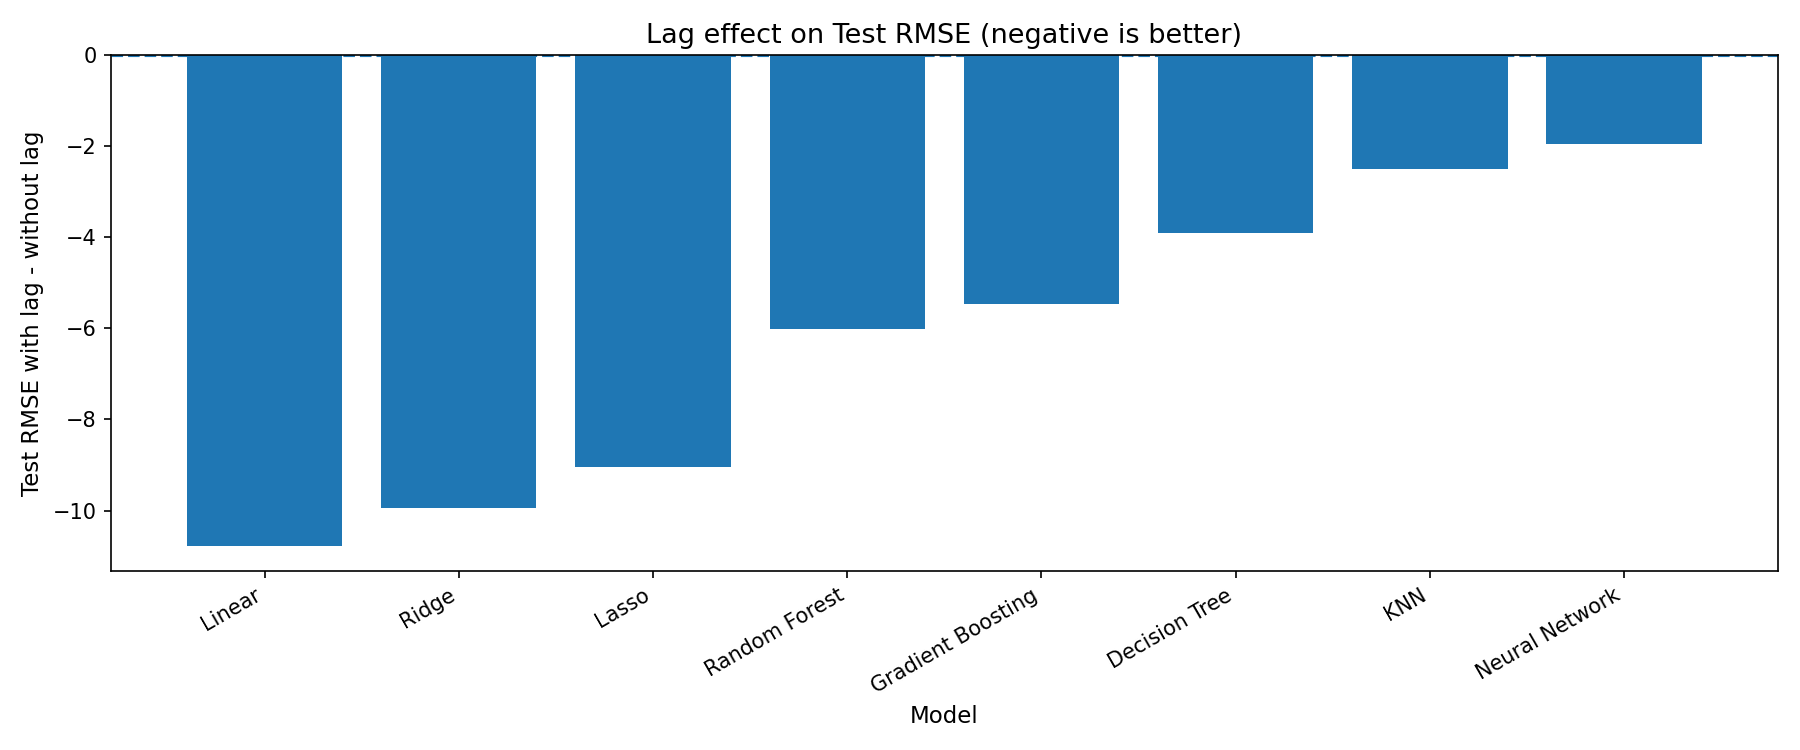
\includegraphics[width=\linewidth]{test_rmse_lag_delta.png}
\caption{Test RMSE decreases for every model when station-specific lag 
features are added. This supports the decision to prioritize temporal 
representation over adding more algorithms.}
\label{fig:lagdelta}
\end{figure}

\subsection{Hyperparameter Tuning Effect}

\begin{table}[htbp]
\caption{Tuning effect: sklearn defaults vs.\ tuned parameters 
(with lag, test set).}
\label{tab:tuning}
\centering
\scriptsize
\begin{tabularx}{\columnwidth}{p{0.32\columnwidth} r r r r}
\toprule
\textbf{Model} & \textbf{RMSE$_{\text{default}}$} & 
\textbf{RMSE$_{\text{tuned}}$} & \textbf{$R^2_{\text{default}}$} & 
\textbf{$R^2_{\text{tuned}}$} \\
\midrule
Gradient Boosting & 23.50 & 22.78 & 0.641 & 0.663 \\
Neural Network    & 24.99 & 24.31 & 0.594 & 0.616 \\
Lasso             & 23.89 & 23.86 & 0.629 & 0.630 \\
\bottomrule
\end{tabularx}
\end{table}

The tuning results show three different patterns. Gradient Boosting 
improved the most: reducing the learning rate from 0.1 to 0.03 and 
increasing the number of trees from 100 to 400 lowered the test RMSE 
by 0.72 points (-3.1\%). This confirms that slower, more conservative 
learning generalizes better for this dataset. The Neural Network also 
improved clearly (-0.68, -2.7\%), but for a different reason: the 
architecture stayed the same (one hidden layer with 128 neurons), 
while the L2 regularization penalty was increased from 0.0001 to 0.1. 
Forcing the network to learn smaller weights reduced overfitting more 
effectively than adding complexity. Lasso barely changed (-0.03, 
-0.1\%), which shows that the sklearn default of $\alpha = 1.0$ was 
already very close to the optimal value for this dataset.

The overall finding is consistent across all three models: the main 
gain came from better regularization and more conservative learning, 
not from increasing model capacity.

\subsection{Result Interpretation}

Gradient Boosting with lag features is the best final model, reaching 
a test RMSE of 22.78, MAE of 16.92, and $R^2$ of 0.663. This means 
that on average, the model's daily rental prediction for a station 
deviates by about 23 rentals from the true value on unseen test data. 
Random Forest is a strong and faster alternative with nearly identical 
accuracy. Lasso shows that a simple regularized linear model becomes 
competitive once the dataset contains the right temporal features.

The most important result is not the winning model alone. Lag features 
improve every model, and better regularization improves tuning results 
across all three algorithm families. Both findings support the same 
conclusion: for this dataset, improving the input representation and 
controlling model complexity matters more than choosing a more 
sophisticated algorithm.

\section{Preliminary Ethical Considerations}

Predicting bike rental demand is generally a low-risk machine learning task. However, we still need to consider some ethical and social effects. 

First, we decided to use only the 20 most used start stations. This was necessary to build a stable first model, but it creates a representation bias. By leaving out smaller stations, our model ignores the demand in areas that might already have fewer services. In a real-world system, this could lead to an unfair distribution of bikes, where less popular neighborhoods get even less attention.

Furthermore, the data we use is completely anonymous and grouped by day and station. This means no personal user information is exposed. If we change our model in the future to use hourly data or specific user types (like registered members or casual users), we must keep this strict privacy standard. 

In future steps of this project, we should also think about the social and economic background of the stations. We must make sure that our model does not systematically disadvantage certain parts of the city.

\section{AI Tool Use}
AI tools were used for drafting support, restructuring text, and helping to standardize code and reporting outputs. The final content, decisions, code execution, result interpretation, and critical reflection were reviewed and organized by the authors.

\end{document}
